\chapter{Membangun Model Prediksi}

\section{Teori}
Praktek teori penunjang yang dikerjakan(nilai 5 per nomor, untuk hari pertama) :
\begin{enumerate}
\item
Jelaskan apa itu binary classification dilengkapi ilustrasi gambar sendiri \\
\textit{Binary Classification} adalah mengklasifikasikan elemen - elemen himpunan menjadi 2 kelompok berdasarkan aturan klasifikasi.
\item
Jelaskan apa itu supervised learning dan unsupervised learning dan clustering dengan ilustrasi gambar sendiri. \\
\begin{itemize}
	\item Supervised Learning
	\par
		\textit{Supervised Learning} adalah suatu pendekatan machine learning yang ditentukan berdasarkan penggunaan dataset, supervised learning menggunakan dataset berlabel atau labeled dataset. Supervised Learning digunakan untuk melakukan klasifikasi data atau memprediksi hasil secara akurat sesuai dengan output berdasarkan pola yang ada didalam data training dan berupa data yang memiliki label yang sudah ditentukan terlebih dahulu. \\
		\begin{figure}[!htbp]
			\centering
			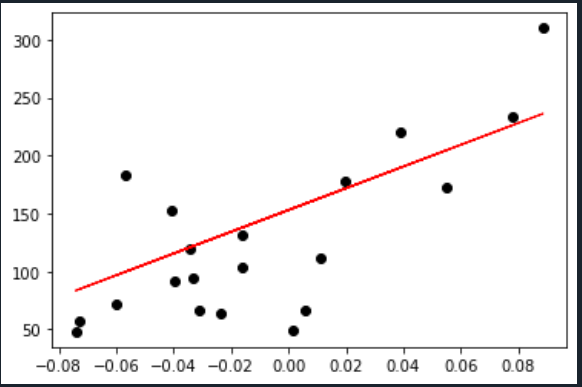
\includegraphics[scale=0.4]{figures/supervised-learning.PNG}
		\end{figure}
		\newpage
	\item Unsupervised Learning
	\par
		\textit{Unsupervised Learning} adalah pendekatan machine learning yang digunakan untuk menganalisa dan juga mengelompokan kumpulan - kumpulan data yang tidak berlabel.\\
		\begin{figure}[!htbp]
			\centering
			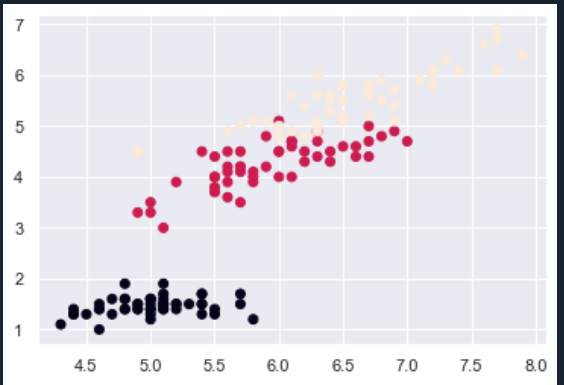
\includegraphics[scale=0.4]{figures/unsupervised-learning.PNG}
		\end{figure}
	\item Clustering
	\par
	\textit{Clustering} adalah sebuah proses pengelompokan data kedalam beberapa cluster sehingga data-data disuatu cluster memiliki kemiripan.\\
	\begin{figure}[!htbp]
		\centering
		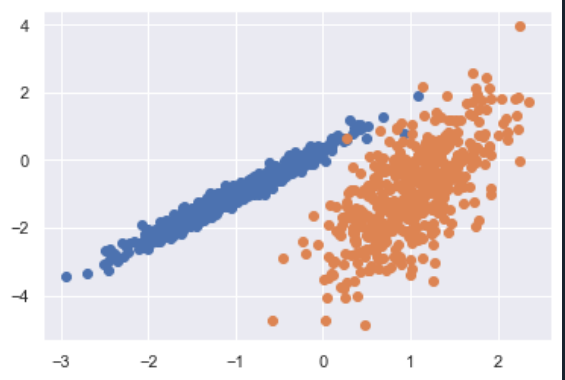
\includegraphics[scale=0.4]{figures/clustering.PNG}
	\end{figure}
	\par
	\item
	Jelaskan apa itu evaluasi dan akurasi dari buku dan disertai ilustrasi contoh dengan gambar sendiri
	\par
	\item 
	\textit{Evaluasi dan Akurasi}
	Evaluasi adalah bagaimana cara agar dapat mengevaluasi seberapa baiknya model bekerja dengan cara mengukur akurasinya.\\
	Akurasi memiliki definisi sebagai persentase kasus yang diklasifikasikan dengan benar.\\
	Kesalahan dari model dapat dianalisi menggunakan confusion matrix.\\
	\par
	\item
	Jelaskan bagaimana cara membuat dan membaca confusion matrix, buat confusion matrix buatan sendiri.
	\par
	\item 
	\textit{Confusion Matrix}\\ 
	1. Import dependencies yang dibutuhkan.\\
	2. Kemudian buat variabel untuk menampung value atau Nilai yang diprediksi.\\
	3. Buat variabel untuk menampung value atau nilai sebenarnya.\\
	4. Kemudian print confusion matrixnya dengan menggunakan variabel dari nilai sebenarnya dan variabel nilai yang diprediksi dengan label misalnya a,b,c.\\
	5. Kemudian print precision dan recall diantara matrix lainnya.
	\begin{figure}[!htbp]
		\centering
		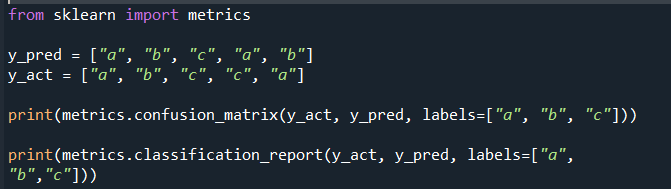
\includegraphics[scale=0.8]{figures/confusionmatrix.PNG}
	\end{figure}
	\begin{figure}[!htbp]
		\centering
		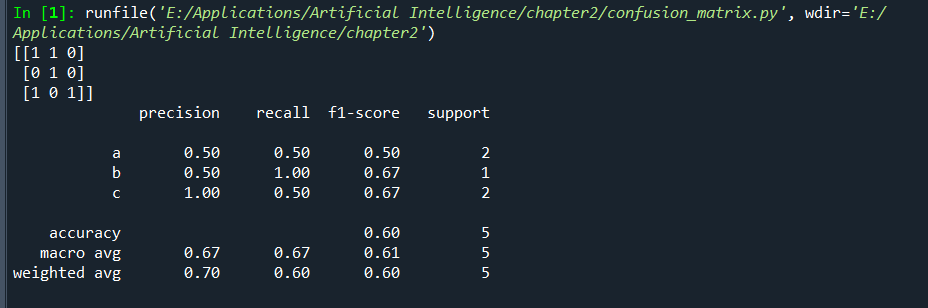
\includegraphics[scale=0.6]{figures/hasilconfusionmatrix.PNG}
	\end{figure}
	\item
	Jelaskan bagaimana K-fold cross validation bekerja dengan gambar ilustrasi contoh buatan sendiri.\\
	\item 
	1. Mengacak dataset secara random.\\
	2. Membagi dataset tersebut kedalam k-group, yaitu sebagai test dataset dan sisanya sebagai training dataset.\\
	3. Pasang model di set pelatihan dan evaluasi di set tes.\\
	4. Simpan skor evaluasi dan buang modelnya.\\
	5. Meringkas keterampilan model menggunakan sampel skor menggunakan model evaluasi.
	\item
	Jelaskan apa itu decision tree dengan gambar ilustrasi contoh buatan sendiri.
	\item 
	\textit{Decision Tree} adalah metode yang digunakan untuk membantu membuat keputusan dengan menggunakan model pohon untuk menampilkan keputusan, kemungkinan resiko, dan lainnya.
	\begin{figure}[!htbp]
		\centering
		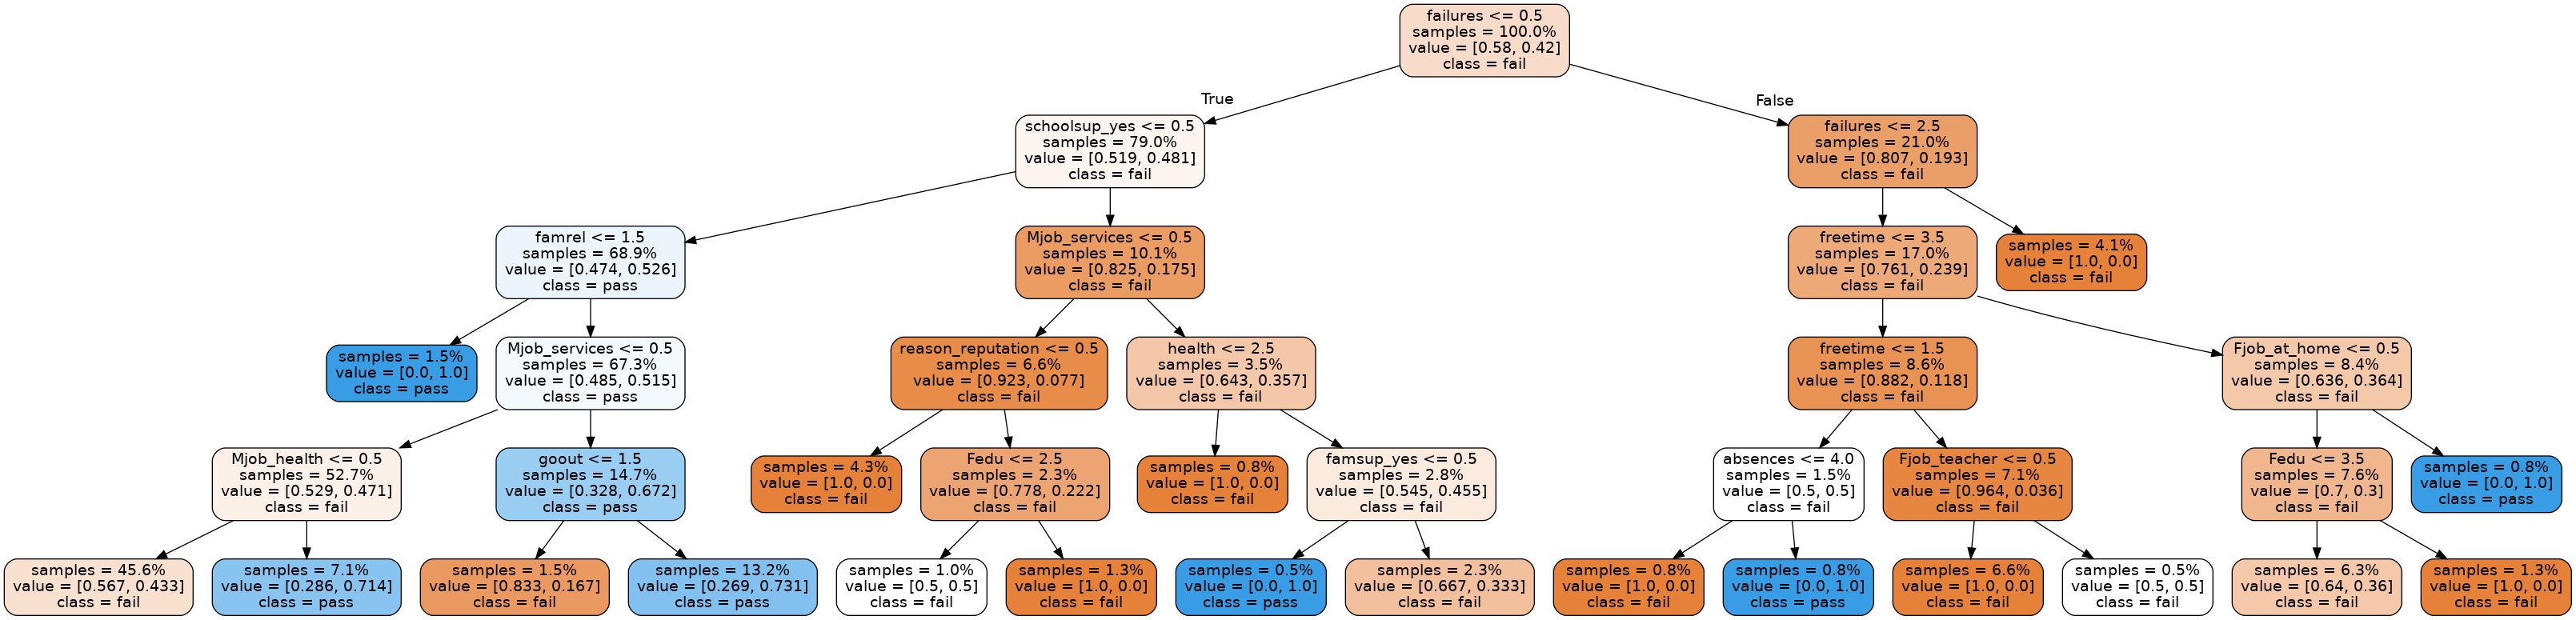
\includegraphics[scale=0.1]{figures/student-performance.PNG}
	\end{figure}
	\item
	Jelaskan apa itu information gain dan entropi dengan gambar ilustrasi buatan sendiri.
	\item 
	\textit{Information Gain} adalah sekumpulan informasi yang didapatkan dari variabel acak.\\
	\textit{Entropi} adalah tingkat keacakan dari informasi yang diperloh dari information gain yang sedang diproses.
\end{itemize}
\end{enumerate}

\section{scikit-learn}
Dataset ambil di https://github.com/PacktPublishing/Python-Artificial-Intelligence-Projects-for-Beginners folder Chapter01.
Tugas anda adalah, dataset ganti menggunakan \textbf{student-mat.csv} dan mengganti semua nama variabel dari kode di bawah ini dengan nama-nama makanan (NPM mod 3=0), kota (NPM mod 3=1), buah (NPM mod 3=2), . Jalankan satu per satu kode tersebut di spyder dengan menggunakan textit{Run current cell}. Kemudian Jelaskan dengan menggunakan bahasa yang mudah dimengerti dan bebas plagiat dan wajib skrinsut dari komputer sendiri masing masing nomor di bawah ini(nilai 5 masing masing pada hari kedua).

\begin{enumerate}

\item
\begin{verbatim}
	#1 Load dataset
	import pandas as pd
	apel = pd.read_csv('student-mat.csv', sep=';')
	len(apel)
\end{verbatim}
	Output :
\begin{figure}[!htbp]
	\centering
	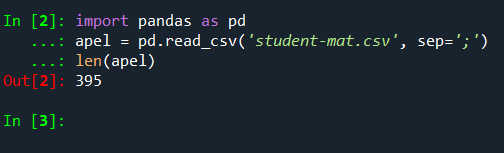
\includegraphics[scale=0.8]{figures/loaddataset1.PNG}
\end{figure}
\item
\begin{verbatim}
	#2 generate binary label (pass)
	# (test grades, each 0-20 pts); threshold for passing is sum>=30
	
	apel['pass'] = apel.apply(lambda row: 1 if (row['G1']+row['G2']+row['G3']) >= 35 else 0, axis=1)
	apel = apel.drop(['G1', 'G2', 'G3'], axis=1)
	apel.head()
\end{verbatim}
	Output :
\begin{figure}[!htbp]
	\centering
	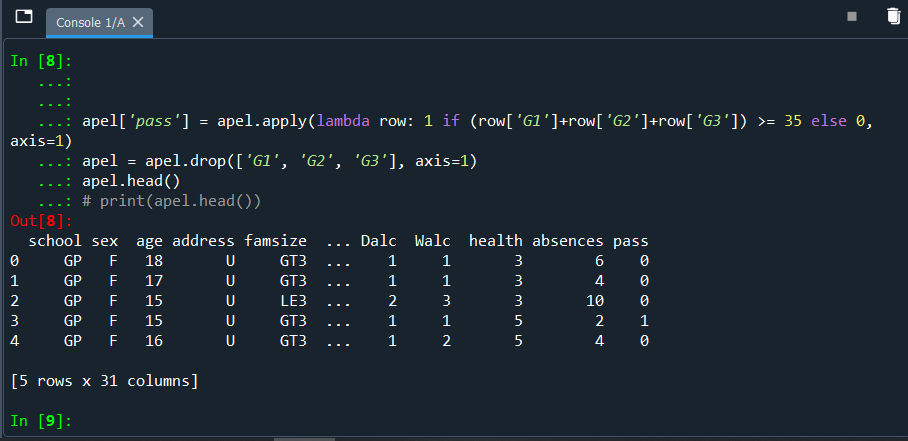
\includegraphics[scale=0.8]{figures/generate_binarylabel.PNG}
\end{figure}
\newpage
\item
\begin{verbatim}
	# 3 use one-hot encoding on categorical columns
	apel = pd.get_dummies(apel, columns=['sex', 'school', 'address', 'famsize', 'Pstatus', 'Mjob', 'Fjob', 
	'reason', 'guardian', 'schoolsup', 'famsup', 'paid', 'activities',
	'nursery', 'higher', 'internet', 'romantic'])
	apel.head()
\end{verbatim}
	Output :
\begin{figure}[!htbp]
	\centering
	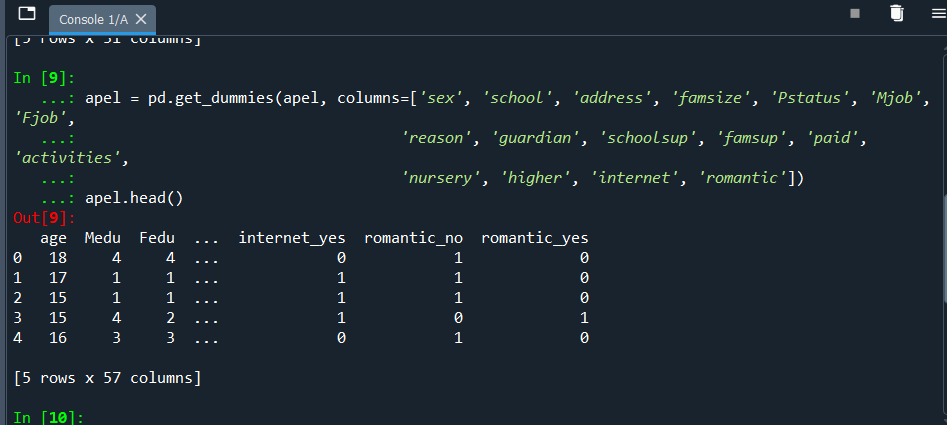
\includegraphics[scale=0.8]{figures/encodingoncategoricalcolumns.PNG}
\end{figure}
\item
\begin{verbatim}
# 4 shuffle rows
apel = apel.sample(frac=1)
#   split traning and testing data
apel_train = apel[:500]
apel_test = apel[:500]

apel_train_att = apel_train.drop(['pass'], axis=1)
apel_train_pass = apel_train['pass']

apel_test_att = apel_test.drop(['pass'], axis=1)
apel_test_pass = apel_test['pass']

apel_att = apel.drop(['pass'], axis=1)
apel_pass = apel['pass']

# number off passing students in whole dataset:
import numpy as np
print("Passing: %d out of %d (%.2f%%)" % (np.sum(apel_pass), len(apel_pass), 
100*float(np.sum(apel_pass)) / len(apel_pass)))
\end{verbatim}
	Output :
\begin{figure}[!htbp]
	\centering
	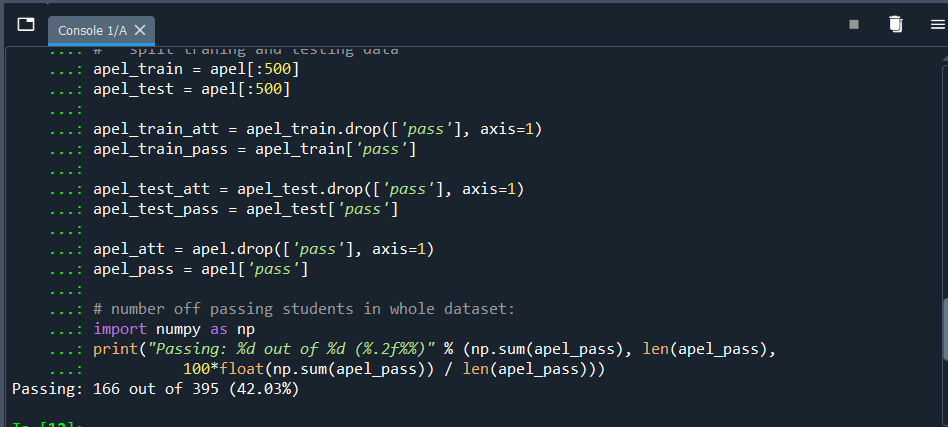
\includegraphics[scale=0.8]{figures/shufflerows.PNG}
\end{figure}
\item 
\begin{verbatim}
	# 5 fit a decision tree
	from sklearn import tree
	semangka = tree.DecisionTreeClassifier(criterion="entropy", max_depth=5)
	semangka = semangka.fit(apel_train_att, apel_train_pass)
\end{verbatim}
\begin{figure}[!htbp]
	\centering
	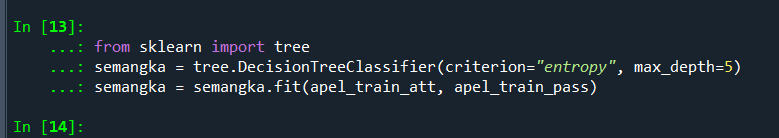
\includegraphics[scale=0.8]{figures/fitdecisontree.PNG}
\end{figure}
\item
\begin{verbatim}
	# 6 visualize tree
	import graphviz
	dot_data = tree.export_graphviz(semangka, out_file=None, label="all", 
	impurity=False, proportion=True,
	feature_names=list(apel_train_att), 
	class_names=["fail", "pass"], 
	filled=True, rounded=True)
	graph = graphviz.Source(dot_data)
	graph
\end{verbatim}
\begin{figure}[!htbp]
	\centering
	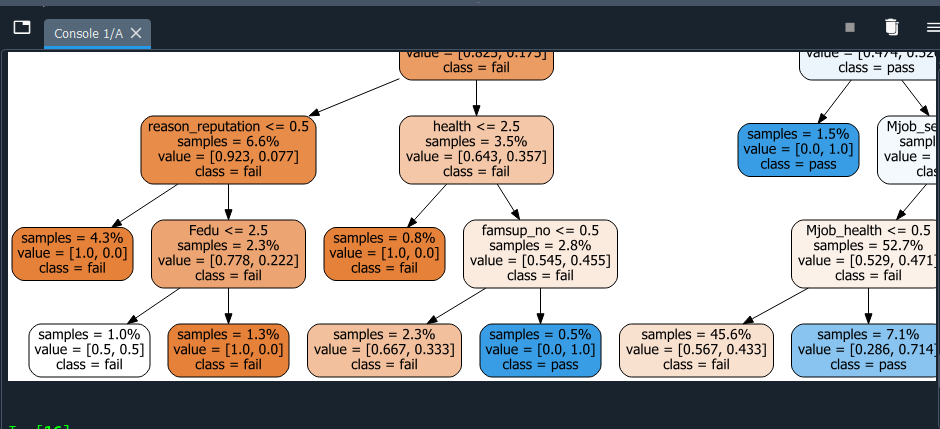
\includegraphics[scale=0.8]{figures/visualizetree.PNG}
\end{figure}
\item
\begin{verbatim}
	# 7 save tree
	tree.export_graphviz(semangka, out_file="student-performance.dot", 
	label="all", impurity=False, 
	proportion=True,
	feature_names=list(apel_train_att), 
	class_names=["fail", "pass"], 
	filled=True, rounded=True)
\end{verbatim}
\begin{figure}[!htbp]
	\centering
	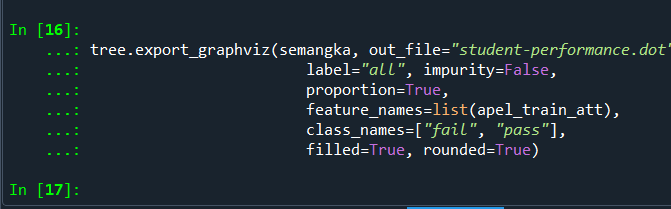
\includegraphics[scale=0.8]{figures/savetree.PNG}
\end{figure}
\item
\begin{verbatim}
	# 8
	semangka.score(apel_test_att, apel_test_pass)
\end{verbatim}
\begin{figure}[!htbp]
	\centering
	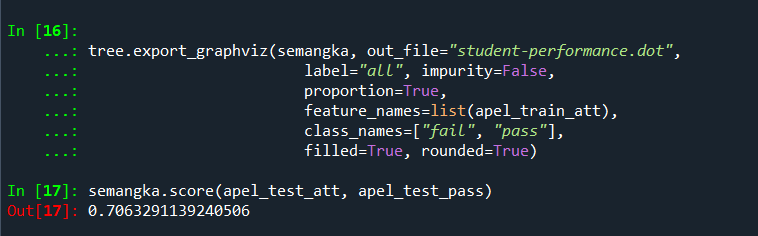
\includegraphics[scale=0.8]{figures/8.PNG}
\end{figure}
\item
\begin{verbatim}
	# 9
	from sklearn.model_selection import cross_val_score
	salak = cross_val_score(semangka, apel_att, apel_pass, cv=5)
	# show average score and +/- two standard deviations away 
	#(covering 95% of scores)
	print("Accuracy: %0.2f (+/- %0.2f)" % (salak.mean(), salak.std() * 2))
\end{verbatim}
\begin{figure}[!htbp]
	\centering
	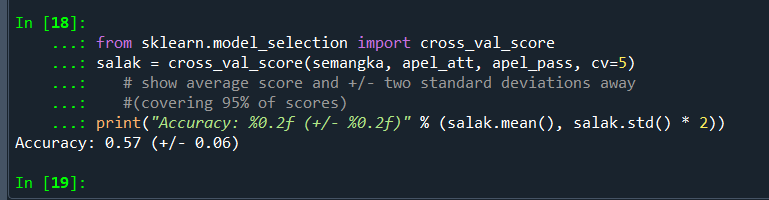
\includegraphics[scale=0.8]{figures/9.PNG}
\end{figure}
\item 
\begin{verbatim}
	# 10
	for max_depth in range(1, 20):
	semangka = tree.DecisionTreeClassifier(criterion="entropy", 
	max_depth=max_depth)
	salak = cross_val_score(semangka, apel_att, apel_pass, cv=5)
	print("Max depth: %d, Accuracy: %0.2f (+/- %0.2f)" % 
	(max_depth, salak.mean(), salak.std() * 2)
	)
\end{verbatim}
\begin{figure}[!htbp]
	\centering
	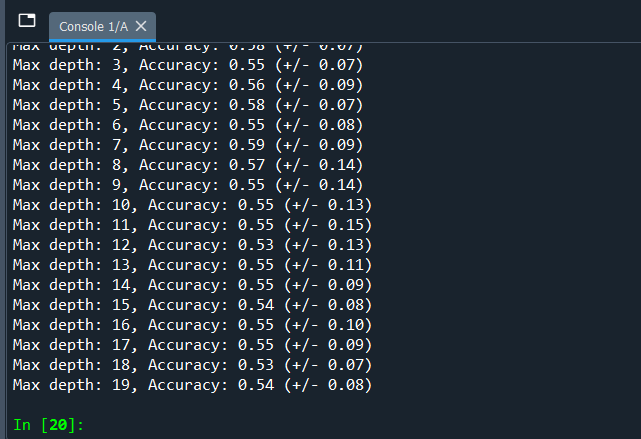
\includegraphics[scale=0.8]{figures/10.PNG}
\end{figure}
\newpage
\item
\begin{verbatim}
	# 11
	depth_acc = np.empty((19,3), float)
	i = 0
	for max_depth in range(1, 20):
	semangka = tree.DecisionTreeClassifier(criterion="entropy", 
	max_depth=max_depth)
	salak = cross_val_score(semangka, apel_att, apel_pass, cv=5)
	depth_acc[i,0] = max_depth
	depth_acc[i,1] = salak.mean()
	depth_acc[i,2] = salak.std() * 2
	i += 1
	depth_acc
\end{verbatim}
\begin{figure}[!htbp]
	\centering
	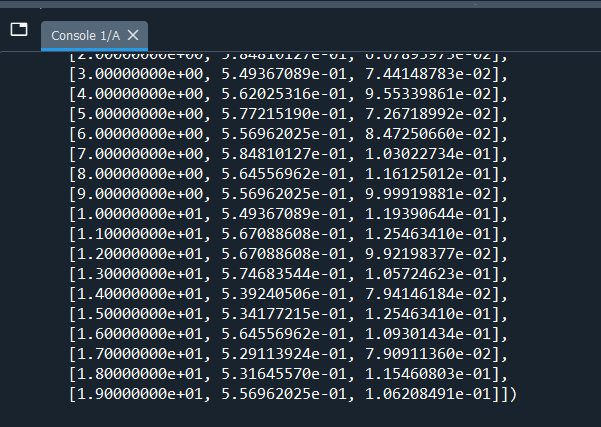
\includegraphics[scale=0.8]{figures/11.PNG}
\end{figure}
\item 
\begin{verbatim}
	# 12
	import matplotlib.pyplot as plt
	fig, ax = plt.subplots()
	ax.errorbar(depth_acc[:,0], depth_acc[:,1], yerr=depth_acc[:,2])
	plt.show()
\end{verbatim}
\begin{figure}[!htbp]
	\centering
	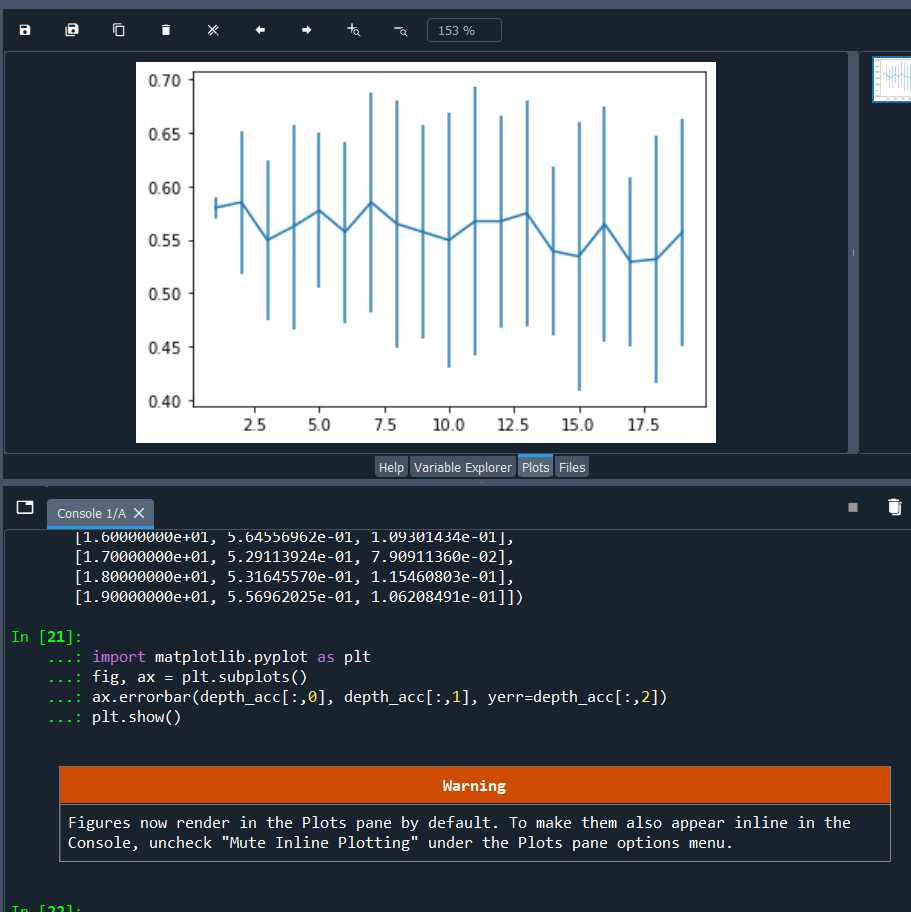
\includegraphics[scale=0.6]{figures/12.PNG}
\end{figure}
\newpage

\end{enumerate}
Link Youtube : https://youtu.be/2aM5RLBPp1c

\section{Penanganan Error}
Dari percobaan yang dilakukan di atas, error yang kita dapatkan di dokumentasikan dan di selesaikan(nilai 5 hari kedua):

\begin{enumerate}
	\item
skrinsut error
\begin{figure}[!htbp]
	\centering
	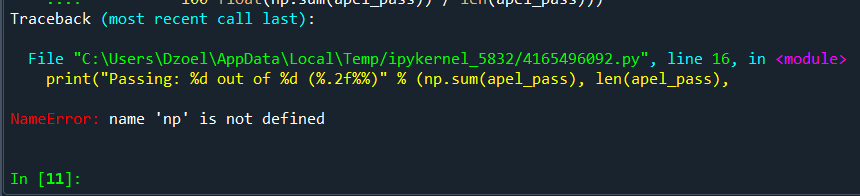
\includegraphics[scale=0.8]{figures/np_not_defined_error.PNG}
\end{figure}
	\item
Tuliskan kode eror dan jenis errornya\\
NameError : name 'np' is not defined
	\item
Solusi pemecahan masalah error tersebut\\
Solusinya adalah import numpy dengan alias np.

\end{enumerate}

